\documentclass[xodstep]{wnspt}

\author      {Filip Świszcz}
\nralbumu    {80236}
\kierunek    {Informatyka}
\specjalnosc {Inżynieria oprogramowania}
\date        {2026}
\miejsce     {Częstochowa,}
\opiekun     {prof. Andrzeja Zbrzeznego}
\opiekunpom  {mgr. inż. Jolanty Podolszańskiej}

\usepackage{amsmath}
\usepackage{amsfonts}
\usepackage{amsthm}
\usepackage{amssymb}
\usepackage[T1]{fontenc}
\usepackage[utf8]{inputenc}
\usepackage[polish]{babel}
\usepackage{polski}
\usepackage{times}
\usepackage{colortbl}
% \usepackage{hyperref}
\usepackage{url}
\usepackage{setspace}
\usepackage{indentfirst}
\usepackage{listingsutf8}
\usepackage{beramono}
\usepackage[section]{placeins}
\usepackage{csquotes}
\usepackage[%
    backend=biber,
    refsegment=section,
    defernumbers=true,
]{biblatex}

\usepackage{fontspec}
\setmainfont{Carlito}

\addbibresource{literatura.bib}

\lstset {
    language=csh,                   % choose the language of the code
    basicstyle=\ttfamily,           % the fonts that are used for the code
    numbers=left,                   % where to put the line-numbers
    numberstyle=\footnotesize,      % the size of the fonts that are used for the line-numbers
    stepnumber=1,                   % the step between two line-numbers. If it's 1 each line will be
    numbersep=5pt,                  % how far the line-numbers are from the code
    showspaces=false,               % show spaces adding particular underscores
    showstringspaces=false,         % underline spaces within strings
    showtabs=false,                 % show tabs within strings adding particular underscores
    frame=single,                   % adds a frame around the code
    tabsize=4,                      % sets default tabsize to 2 spaces
    captionpos=b,                   % sets the caption-position to bottom
    breaklines=true,                % sets automatic line breaking
    breakatwhitespace=false,        % sets if automatic breaks should only happen at whitespace
    escapeinside={\%*}{*)}          % if you want to add a comment within your code 
}

\newcommand{\file}[1]{\texttt{#1}}
\newcommand{\dir}[1]{\texttt{#1}}
\newcommand{\func}[1]{\lstinline|#1()|}
\newcommand{\var}[1]{\lstinline|#1|}

\newcommand{\R}{mathbb{R}}

\renewcommand{\lstlistlistingname}{Spis listingów}
\renewcommand{\lstlistingname}{Listing}

\newtheorem{lemat}{Lemat}
\newtheorem{twierdzenie}{Twierdzenie}

\title{Interaktywna wizualizacja systemu słonecznego \\{~} Interactive visualization of the solar system}

\frenchspacing

\begin{document}

% streszczenie
\begin{abstract}
    Aplikacja desktopowa będąca symulatorem systemu słonecznego ma na celu dostarczenie interaktywnego narzędzia edukacyjnego, pozwalającego użytkownikowi na eksplorację kosmosu w czasie rzeczywistym. Program umożliwia swobodne poruszanie się w przestrzeni trójwymiarowej, manipulację upływem czasu oraz obserwację ruchu planet po orbitach obliczonych na podstawie praw fizyki. W pracy omówiono proces projektowania silnika graficznego od podstaw w języku C, implementację własnej biblioteki matematycznej, obsługę shaderów oraz stworzenie autorskiego formatu plików modeli (.orb) w celu optymalizacji ładowania danych.
\end{abstract}

% słowa kluczowe
\keywords{C, GLSL, OpenGL, GLFW, GLEW, Git, Make, Symulacja fizyczna}

\maketitle
\onehalfspacing

% wstęp
\introduction
Grafika komputerowa i symulacje fizyczne stanowią jeden z najbardziej dynamicznie rozwijających się obszarów informatyki. Choć współczesny rynek oprogramowania zdominowany jest przez zaawansowane silniki gier (takie jak Unity czy Unreal Engine), które automatyzują większość procesów renderowania \cite{book_gregory_game_engine}, dogłębne zrozumienie zasad działania potoku graficznego wymaga zejścia do poziomu niskopoziomowego programowania \cite{book_moller_real_time_rendering}.

Celem niniejszej pracy inżynierskiej jest zaprojektowanie i implementacja interaktywnej wizualizacji Układu Słonecznego („SOLAR”), wykonanej w języku C z wykorzystaniem biblioteki graficznej OpenGL. Projekt ten nie jest jedynie wizualizacją astronomiczną, lecz przede wszystkim próba stworzenia autorskiego, minimalistycznego silnika graficznego. Kluczowym założeniem pracy jest rezygnacja z gotowych bibliotek wspomagających obliczenia matematyczne (takich jak GLM) na rzecz własnej implementacji algebry liniowej oraz stworzenie dedykowanego formatu plików modeli 3D (.orb), zoptymalizowanego pod kątem czasu ładowania i zużycia pamięci.

Wybór języka C podyktowany był chęcią uzyskania pełnej kontroli nad zarządzaniem pamięcią oraz wydajnością aplikacji, co jest kluczowe w systemach czasu rzeczywistego. Aplikacja umożliwia użytkownikowi swobodną eksplorację przestrzeni kosmicznej, manipulację upływem czasu oraz obserwację ruchu planet po orbitach wyznaczonych zgodnie z prawami mechaniki nieba.

Praca została podzielona na pięć rozdziałów. W rozdziale pierwszym przedstawiono podstawy teoretyczne, analizę istniejących rozwiązań oraz specyfikację wymagań projektowych. Rozdział drugi charakteryzuje środowisko programistyczne i uzasadnia wybór technologii (język C, OpenGL). Rozdział trzeci omawia ogólną architekturę systemu, cykl życia aplikacji oraz organizację struktur danych. Rozdział czwarty stanowi dokumentację techniczną warstwy silnika, obejmującą autorską bibliotekę matematyczną, podsystem renderowania oraz zarządzanie zasobami. Całość zamyka rozdział piąty poświęcony implementacji właściwej symulacji, w tym modelowi fizycznemu ciał niebieskich, systemowi czasu oraz interfejsowi użytkownika.

% \cite{
%     book_gregory_game_engine,
%     book_moller_real_time_rendering,
%     book_wright_opengl_superbible,
%     book_bate_astrodynamics,
%     book_lengyel_math_3d,
%     article_leblanc_mechanics,
%     article_fowler_fnv_hash,
%     article_nijenhuis_kepler_equation,
%     article_berger_custom_allocators,
%     article_wilson_memory_management,
%     online_learnopengl,
%     online_opengl_spec_41,
%     online_glfw_docs,
%     online_glew_docs,
%     online_nasa_jpl_horizons,
%     online_stb_image,
% }

\input{chapters/chapter1}
\chapter{Środowisko i narzędzia wytwórcze}

 Wybór odpowiedniego zestawu technologii i narzędzi programistycznych jest kluczowym etapem realizacji każdego projektu inżynierskiego. 
 W przypadku silnika graficznego i symulacji fizycznej, priorytetem była wydajność, przenośność oraz możliwość bezpośredniej interakcji ze sprzętem graficznym.
  W niniejszym rozdziale omówiono język programowania, biblioteki oraz narzędzia wykorzystane w procesie tworzenia aplikacji „SOLAR”.

    % 2.1
    \section{Język programowania C}

     Jako podstawowe narzędzie implementacji wybrano język C w standardzie C99.
     Decyzja ta, choć może wydawać się nietypowa w dobie wysokopoziomowych języków obiektowych, była podyktowana specyficznymi wymaganiami inżynierii gier i symulacji fizycznych. 
     Język C oferuje bezkompromisową wydajność oraz niskopoziomowy dostęp do pamięci operacyjnej, co jest krytyczne przy przetwarzaniu tysięcy wierzchołków i obliczaniu fizyki orbitalnej w każdej klatce obrazu. 
     W przeciwieństwie do języków wyposażonych w automatyczne odśmiecanie pamięci (Garbage Collection), C wymusza na programiście ręczne zarządzanie alokacją i dealokacją zasobów. 
     W projekcie wykorzystano ten fakt do zaimplementowania własnego, zoptymalizowanego mechanizmu zarządzania pamięcią, opartego na koncepcji alokatora liniowego (tzw. Memory Arena) \cite{article_berger_custom_allocators, article_wilson_memory_management}.
     Rozwiązanie to, zdefiniowane w module \file{d\_arena}, pozwala na wydzielenie dużego, ciągłego bloku pamięci i przydzielanie w nim przestrzeni dla poszczególnych obiektów, co drastycznie minimalizuje narzut czasowy wywołań systemowych oraz niemal całkowicie eliminuje zjawisko fragmentacji sterty, krytyczne dla aplikacji działających w czasie rzeczywistym.

     \newpage

    % 2.2
    \section{Biblioteka graficzna OpenGL 4.1 Core Profile}

     Warstwa wizualna aplikacji została oparta na bibliotece OpenGL w wersji 4.1 Core Profile. Jest to otwarty standard interfejsu programistycznego, służący do generowania grafiki dwu- i trójwymiarowej. Wybór wersji 4.1 stanowił świadomy kompromis pomiędzy dostępem do nowoczesnych funkcji a kompatybilnością sprzętową. Wersja ta jest ostatnią natywnie wspieraną przez systemy operacyjne macOS, co zapewnia przenośność aplikacji między platformami Windows, Linux i Apple bez konieczności modyfikacji kodu źródłowego. Zastosowanie profilu rdzennego (Core Profile) \cite{online_opengl_spec_41} oznacza całkowitą rezygnację z przestarzałego modelu "Fixed Function Pipeline" na rzecz w pełni programowalnego potoku renderującego \cite{book_wright_opengl_superbible}. Wymusiło to implementację własnych shaderów w języku GLSL (OpenGL Shading Language), odpowiedzialnych za transformację geometrii oraz obliczanie oświetlenia pikseli bezpośrednio na procesorze graficznym (GPU). Takie podejście pozwala na uzyskanie znacznie wyższej wydajności i elastyczności w kreowaniu efektów wizualnych niż w przypadku gotowych rozwiązań.

   \newpage

    % 2.3
    \section{Biblioteki pomocnicze}

     OpenGL jest jedynie specyfikacją API graficznego i nie zawiera funkcji do obsługi systemu operacyjnego (tworzenie okna, obsługa klawiatury) ani ładowania plików. W związku z tym wykorzystano zestaw lekkich, specjalizowanych bibliotek.

        \subsection{GLFW}

         Biblioteka GLFW \cite{online_glfw_docs} posłużyła do utworzenia kontekstu OpenGL, zarządzania oknem aplikacji oraz obsługi urządzeń wejścia (mysz, klawiatura).
         W pliku \texttt{g\_game.c} wykorzystano funkcje takie jak glfwGetCursorPos do sterowania kamerą oraz glfwGetKey do obsługi poruszania się w przestrzeni. GLFW zapewnia abstrakcję warstwy systemowej, dzięki czemu aplikacja może być kompilowana zarówno na systemach Windows, Linux, jak i macOS.

        \subsection{GLEW / GLCoreARB}

         Ze względu na specyfikę ładowania funkcji OpenGL, które są dostarczane przez sterowniki karty graficznej, konieczne jest użycie mechanizmu ładującego wskaźniki do tych funkcji.

         \bigbreak

         - Na systemach Windows/Linux wykorzystano bibliotekę GLEW \cite{online_glew_docs}

         - Na systemie macOS (zdefiniowanym makrem \_\_APPLE\_\_) wykorzystano nagłówki GLCoreARB

        \subsection{stb\_image}
        
         Do wczytywania tekstur (formaty .jpg, .png) użyto biblioteki \texttt{stb\_image} \cite{online_stb_image}. Jest to biblioteka typu "header-only" (zawarta w jednym pliku nagłówkowym), co znacząco upraszcza proces kompilacji. W module \texttt{d\_util.c} funkcja stbi\_load dekoduje pliki graficzne do surowej tablicy bajtów, która następnie jest przesyłana do pamięci karty graficznej funkcją glTexImage2D.

   \newpage

    % 2.4
    \section{Narzędzia budowania i systemy kontroli wersji}

     Proces wytwórczy oprogramowania wspierany był przez standardowe narzędzia inżynierskie.

        \subsection{Make}

         Do automatyzacji procesu kompilacji wykorzystano narzędzie Make. Plik konfiguracyjny Makefile definiuje reguły kompilacji poszczególnych modułów (.c) do plików obiektowych (.o), a następnie ich linkowania w plik wykonywalny. Pozwala to na szybką rekompilację tylko tych części kodu, które uległy zmianie, oraz łatwe zarządzanie flagami kompilatora i linkera (np. -lGL -lglfw).

        \subsection{Git}

         Zarządzanie kodem źródłowym odbywało się przy użyciu systemu kontroli wersji Git. Umożliwiło to śledzenie historii zmian, eksperymentowanie z nowymi funkcjami (np. implementacja formatu .orb) na osobnych gałęziach (branch) oraz zabezpieczenie kodu przed utratą. Struktura repozytorium została podzielona na katalogi logiczne: src (kod źródłowy), assets (zasoby), shader (kody shaderów) oraz tools (narzędzia pomocnicze).
\input{chapters/chapter3}
\input{chapters/chapter4}
\chapter{Implementacja logiki symulacji}
 Niniejszy rozdział skupia się na implementacji zasad fizyki orbitalnej, systemie zarządzania czasem oraz mechanizmach interakcji użytkownika z wirtualnym Układem Słonecznym.

    % 5.1
    \section{Fizyka i model danych ciał niebieskich (\file{r\_physics})}
     Model fizyczny aplikacji został zaprojektowany w oparciu o uproszczoną mechanikę nieba, wykorzystującą parametry orbitalne do deterministycznego wyznaczania pozycji ciał niebieskich w dowolnym momencie czasu.

        % 5.1.1
        \subsection{Struktura planety (\file{planet\_t})}

         \begin{itemize}
             \item[---] \textbf{Dane identyfikacyjne i wizualne:} Nazwa planety (\var{name}) oraz kolor bazowy (\var{color}) wykorzystywany przez elementy interfejsu.
             \item[---] \textbf{Elementy orbitalne Keplera:}
             \begin{itemize}
                 \item[---] \var{orbit.semi_major_axis}: Średnia odległość od ciała centralnego
                 \item[---] \var{orbit.period_orbital}: Czas pełnego obiegu wokół orbity (rok gwiazdowy)
                 \item[---] \var{orbit.mean_anomaly_epoch}: Przesunięcie początkowe, pozwalające ustalić pozycję planety w epoce startowej (np. J2000)
                 \item[---] \var{inclination}: Kąt nachylenia płaszczyzny orbity do płaszczyzny odniesienia (ekliptyki)
                 \item[---] \var{long_asc_node}: Kąt określający orientację orbity w płaszczyźnie odniesienia
             \end{itemize}
             \item[---] \textbf{Parametry rotacyjne:} \var{period_rotation} (okres obrotu wokół własnej osi) oraz \var{obliquity} (nachylenie osi obrotu).
             \item[---] \textbf{Hierarchia:} Wskaźnik \var{struct planet *parent}, umożliwiający tworzenie układów zależnych (np. Księżyc krążący wokół Ziemi, która krąży wokół Słońca).
         \end{itemize}

         \newpage

        % Rysunek 5.1 Schemat "Elementy orbitalne Keplera"

        \vspace{1em}
        \begin{table}[htpb]
        \centering
        \caption{Wybrane parametry fizyczne i orbitalne ciał niebieskich zaimplementowane w kodzie symulacji}
        \label{tab:planets_data}
        \resizebox{\textwidth}{!}{% Skalowanie tabeli do szerokości strony
        \begin{tabular}{|l|r|r|r|r|r|}
        \hline
        \textbf{Ciało niebieskie} & \textbf{Promień równikowy [km]} & \textbf{Półoś wielka [km]} & \textbf{Mimośród} & \textbf{Okres orbitalny [dni]} & \textbf{Inklinacja [$^\circ$]} \\ \hline
        Słońce  & 695 700.0 & 0.0         & 0.000000 & 0.0     & 0.000  \\ \hline
        Merkury & 2 439.7   & 57 909 227  & 0.205630 & 87.97   & 7.005  \\ \hline
        Wenus   & 6 051.8   & 108 209 475 & 0.006772 & 224.70  & 3.395  \\ \hline
        Ziemia  & 6 371.0   & 149 597 870 & 0.016708 & 365.26  & 0.000  \\ \hline
        Mars    & 3 389.5   & 227 939 200 & 0.093400 & 686.98  & 1.850  \\ \hline
        Jowisz  & 69 911.0  & 778 340 821 & 0.048498 & 4332.59 & 1.304  \\ \hline
        Saturn  & 58 232.0  & 1 426 666 422 & 0.055546 & 10759.22& 2.485  \\ \hline
        Uran    & 25 362.0  & 2 870 658 186 & 0.047318 & 30685.40& 0.773  \\ \hline
        Neptun  & 24 622.0  & 4 498 396 441 & 0.008606 & 60189.00& 1.770  \\ \hline
        Pluton  & 1 188.3   & 5 906 380 000 & 0.248800 & 90560.00& 17.160 \\ \hline
        \end{tabular}%
        }
        \end{table}

        % 5.1.2
        \subsection{Integracja z grafiką}
         Kluczowym aspektem architektury jest sposób połączenia warstwy fizycznej z warstwą prezentacji.
         Zamiast dziedziczenia, zastosowano kompozycję: struktura \var{planet\_t} zawiera wskaźnik \var{object\_t *object}.
        
         Obiekt graficzny (\var{object\_t}) przechowuje siatkę geometryczną, teksturę i shader, ale nie posiada wiedzy o swojej pozycji w kontekście astronomicznym.
         W każdej klatce symulacji, funkcja aktualizująca stan planety oblicza nową pozycję, a następnie modyfikuje macierz modelu (\var{u_Model}) powiązanego obiektu graficznego.

         Dzięki temu rozwiązaniu, renderer pozostaje niezależnym modułem, który jedynie "wyświetla" to, co obliczyła fizyka.
         Pozwala to również na łatwą zmianę reprezentacji wizualnej planety (np. podmianę modelu na dokładniejszy) bez ingerencji w kod fizyki.

         \newpage

        \vspace{1em}
        \begin{lstlisting}[language=C, caption={Budowa finalnej macierzy modelu w pętli głównej poprzez sekwencyjne nakładanie transformacji: nachylenia osi (obliquity), rotacji dobowej, skalowania oraz pozycji orbitalnej}, label={lst:model_matrix}]
    mat4_t model = mat4(1.0f);

    // Aplikacja nachylenia osi i rotacji planety
    model = r_rotate(model, context.scene.planets[i].obliquity * (180.0f / R_PI), vec3(0.0f, 0.0f, 1.0f));
    model = r_rotate(model, context.scene.planets[i].state.rotation * (180.0f / R_PI), vec3(0.0f, 1.0f, 0.0f));

    // Aplikacja skali fizycznej
    float scale = (i == 0) ? 0.8f : 1.6f;
    model = r_scale(model, vec3_mul(vec3(
        context.scene.planets[i].radius_equatorial * scale, 
        context.scene.planets[i].radius_equatorial * scale, 
        context.scene.planets[i].radius_equatorial * scale
    ), R_PHYSICS_PLANET_SCALE));

    // Aplikacja pozycji orbitalnej z przestrzeni r_physics
    model = r_translate(model, vec3_mul(context.scene.planets[i].state.position, R_PHYSICS_ORBIT_SCALE));

    r_set_mat4(context.scene.planets[i].object -> shader, "u_Model", model);
        \end{lstlisting}

         \newpage

        % 5.1.3
        \subsection{Algorytm pozycyjny}
         Wyznaczanie pozycji ciał niebieskich realizowane jest przez funkcję \func{r\_physics\_planet\_state\_update} oraz pomocniczą funkcję \func{r\_physics\_orbit\_to\_local}. 
         Proces ten przebiega w następujących krokach:

         \begin{enumerate}
             \item \textbf{Obliczenie anomalii średniej:} Na podstawie aktualnego czasu symulacji (\var{time}) wyznaczany jest kąt na orbicie (\var{orbit\_angle}). Uwzględnia się przy tym okres orbitalny oraz fazę początkową.
             \item \textbf{Wyznaczenie pozycji na płaszczyźnie orbity:} Współrzędne obliczane są przy założeniu orbity kołowej (dla uproszczenia mimośrodów bliskich zeru):
                 \begin{equation}
                 x = r \cdot \cos(\theta), \quad z = r \cdot \sin(\theta)
                 \end{equation}
             \item \textbf{Transformacja do układu lokalnego:} Pozycja jest poddawana obrotom zgodnie z parametrami orbitalnymi. Najpierw następuje obrót o kąt inklinacji wokół osi X, a następnie obrót o kąt węzła wstępującego wokół osi Y.
             \item \textbf{Uwzględnienie hierarchii:} Jeśli planeta posiada rodzica (pole parent nie jest NULL), do obliczonej pozycji dodawany jest wektor pozycji rodzica. Pozwala to na poprawne symulowanie układów satelitarnych.
         \end{enumerate}

         \newpage

         \textbf{Algorytm Newtona-Raphsona}
         
         \bigbreak

         Podstawowym wyzwaniem w modelu keplerowskim jest wyznaczenie anomalii mimośrodowej ($E$) na podstawie anomalii średniej ($M$) oraz mimośrodu orbity ($e$).
         Zależność tę opisuje równanie Keplera:

         \begin{equation}
         M = E - e * \sin(E)
         \end{equation}

         Równanie to jest równaniem przestępnym i nie posiada jawnego rozwiązania analitycznego.
         W celu jego rozwiązania w czasie rzeczywistym, w module fizycznym (\func{\_r\_physics\_kepler\_solve}) zaimplementowano numeryczną metodę Newtona-Raphsona.
         W kolejnych iteracjach pętli, przybliżona wartość $E$ jest korygowana zgodnie ze wzorem:

         \begin{equation}
         E_{n+1} = E_n - \frac{E_n - e \sin(E_n) - M}{1 - e \cos(E_n)}
         \end{equation}

         Dzięki bardzo szybkiemu tempu zbieżności tej metody, wystarczy zaledwie kilka iteracji (w implementacji założono stałą liczbę 5 kroków), aby uzyskać precyzję zmiennoprzecinkową wystarczającą dla poprawnego i płynnego pozycjonowania ciał niebieskich na orbitach.

        \vspace{1em}
        \begin{lstlisting}[language=C, caption={Implementacja algorytmu Newtona-Raphsona do numerycznego rozwiązywania równania Keplera}, label={lst:kepler_solve}]
        double _r_physics_kepler_solve(double mean, double eccentric) {
            double E = mean;
            for (uint32_t i = 0; i < 5; i++) {
                double delta = E - eccentric * sin(E) - mean;
                E = E - delta / (1.0 - eccentric * cos(E));
            }
            return E;
        }
        \end{lstlisting}

        \newpage

    % 5.2
    \section{System czasu i kalendarza}
     Zarządzanie czasem jest krytycznym elementem symulacji astronomicznej, pozwalającym na obserwację zjawisk zachodzących w skali od minut do stuleci.

        % 5.2.1
        \subsection{Obsługa czasu rzeczywistego i symulowanego}
         Wewnętrzny zegar symulacji (\var{context.scene.clock.time}) reprezentowany jest przez zmienną typu double, przechowującą liczbę sekund, jakie upłynęły od epoki J2000 (1 stycznia 2000, 12:00 TT).
         Taka reprezentacja zapewnia wysoką precyzję i ułatwia obliczenia astronomiczne.

         W celu prezentacji daty użytkownikowi, zaimplementowano funkcję \func{r\_physics\_clock\_to\_tm}, która konwertuje czas liniowy na strukturę kalendarzową \var{struct tm} (rok, miesiąc, dzień).
         Wykorzystano w tym celu standardowe funkcje biblioteki C (\var{mktime, localtime_r}), traktując rok 2000 jako punkt odniesienia.

        % 5.2.2
        \subsection{Mechanizm sterowania upływem czasu}
         Aplikacja umożliwia dynamiczną zmianę prędkości upływu czasu. 
         Zaimplementowano to przy użyciu tablicy prędkości \var{speeds} oraz kursora wskazującego na aktualnie wybrany mnożnik. 
         Tablica zawiera wartości od ujemnych (cofanie czasu), przez zero (pauza), aż po wartości dodatnie symulujące upływ lat w ciągu sekund.

         W każdej klatce pętli głównej, czas symulacji jest inkrementowany o wartość: \var{context.fps.time_between_frames} * \var{speeds[cursor]}.
         
         Sterowanie odbywa się za pomocą klawiszy klawiatury (H - zwolnienie/cofanie, K - przyspieszenie, J - reset do czasu rzeczywistego), co pozwala użytkownikowi na płynną nawigację w chronologii Układu Słonecznego.

        \vspace{1em}
        \begin{table}[htpb]
        \centering
        \caption{Skróty klawiszowe umożliwiające manipulację kalendarzem symulacji}
        \label{tab:time_controls}
        \begin{tabular}{|c|p{10cm}|}
        \hline
        \textbf{Klawisz} & \textbf{Akcja (zmiana w tablicy \var{speeds})} \\ \hline
        \textbf{H} & Zmniejszenie mnożnika upływu czasu (pozwala na zwolnienie biegu wydarzeń, zatrzymanie, aż do płynnego cofania symulacji). \\ \hline
        \textbf{K} & Zwiększenie mnożnika upływu czasu (przyspieszenie symulacji, pozwalające zaobserwować ruch powolnych planet zewnętrznych). \\ \hline
        \textbf{J} & Błyskawiczny reset wskaźnika (\var{cursor = 17}) do domyślnego upływu czasu. \\ \hline
        \end{tabular}
        \end{table}

        \vspace{1em}
        \begin{table}[htpb]
        \centering
        \caption{Pełne zestawienie dostępnych mnożników upływu czasu (wartości tablicy \var{speeds}), po których porusza się kursor sterowania}
        \label{tab:time_speeds}
        \begin{tabular}{|c|l|l|}
        \hline
        \textbf{Indeks (kursor)} & \textbf{Upływ czasu w grze (na 1 sekundę rzeczywistą)} & \textbf{Reprezentacja w kodzie symulacji} \\ \hline
        0  & $-1$ rok (szybkie cofanie) & \var{-R\_PHYSICS\_YEAR\_SECONDS} \\ \hline
        1  & $-10$ miesięcy             & \var{-10 * R\_PHYSICS\_MONTH\_SECONDS} \\ \hline
        2  & $-1$ miesiąc               & \var{-R\_PHYSICS\_MONTH\_SECONDS} \\ \hline
        3  & $-10$ dni                  & \var{-10 * R\_PHYSICS\_DAY\_SECONDS} \\ \hline
        4  & $-1$ dzień                 & \var{-R\_PHYSICS\_DAY\_SECONDS} \\ \hline
        5  & $-10$ godzin               & \var{-10 * R\_PHYSICS\_HOUR\_SECONDS} \\ \hline
        6  & $-1$ godzina               & \var{-R\_PHYSICS\_HOUR\_SECONDS} \\ \hline
        7  & $-10$ minut                & \var{-10 * R\_PHYSICS\_MINUTE\_SECONDS} \\ \hline
        8  & $-1$ minuta                & \var{-R\_PHYSICS\_MINUTE\_SECONDS} \\ \hline
        9  & $-10$ sekund               & \var{-10.0} \\ \hline
        10 & $-1$ sekunda (czas wstecz) & \var{-1.0} \\ \hline
        11 & $1$ sekunda (czas realny)  & \var{1.0} \\ \hline
        12 & $10$ sekund                & \var{10.0} \\ \hline
        13 & $1$ minuta                 & \var{R\_PHYSICS\_MINUTE\_SECONDS} \\ \hline
        14 & $10$ minut                 & \var{10 * R\_PHYSICS\_MINUTE\_SECONDS} \\ \hline
        15 & $1$ godzina                & \var{R\_PHYSICS\_HOUR\_SECONDS} \\ \hline
        16 & $10$ godzin                & \var{10 * R\_PHYSICS\_HOUR\_SECONDS} \\ \hline
        \textbf{17} & \textbf{1 dzień (domyślny startowy)} & \textbf{\var{R\_PHYSICS\_DAY\_SECONDS}} \\ \hline
        18 & $10$ dni                   & \var{10 * R\_PHYSICS\_DAY\_SECONDS} \\ \hline
        19 & $1$ miesiąc                & \var{R\_PHYSICS\_MONTH\_SECONDS} \\ \hline
        20 & $10$ miesięcy              & \var{10 * R\_PHYSICS\_MONTH\_SECONDS} \\ \hline
        21 & $1$ rok (szybkie przewijanie) & \var{R\_PHYSICS\_YEAR\_SECONDS} \\ \hline
        \end{tabular}
        \end{table}

    % 5.3
    \section{Interfejs i interakcja w przestrzeni 3D}
     Ze względu na specyficzną skalę kosmosu (ogromne odległości i stosunkowo małe obiekty), konieczne było zaprojektowanie elementów wizualnych ułatwiających orientację w przestrzeni.

        % 5.3.1
        \subsection{Wizualizacja orbit}
         Linie orbit nie są częścią modeli 3D, lecz są generowane proceduralnie podczas inicjalizacji sceny (\func{\_g\_game\_ui\_orbits\_init}). 
         Algorytm iteruje przez kąt od $0$ do $2\pi$ z zadanym krokiem, wykorzystując tę samą funkcję fizyczną \func{r\_physics\_orbit\_to\_local}, która służy do pozycjonowania planet.

         Wygenerowane wierzchołki są przesyłane do osobnego bufora VBO i rysowane jako prymityw \var{GL_LINE_LOOP}. 
         Dzięki temu orbity idealnie pokrywają się z trajektorią ruchu planet, uwzględniając ich inklinację i ekscentryczność.
         Do ich renderowania użyto dedykowanego shadera (\file{orbit.vs}, \file{orbit.fs}), który umożliwia nadanie im stałego koloru i jasności, niezależnie od oświetlenia słonecznego. 

        \begin{figure}[htpb]
            \centering
            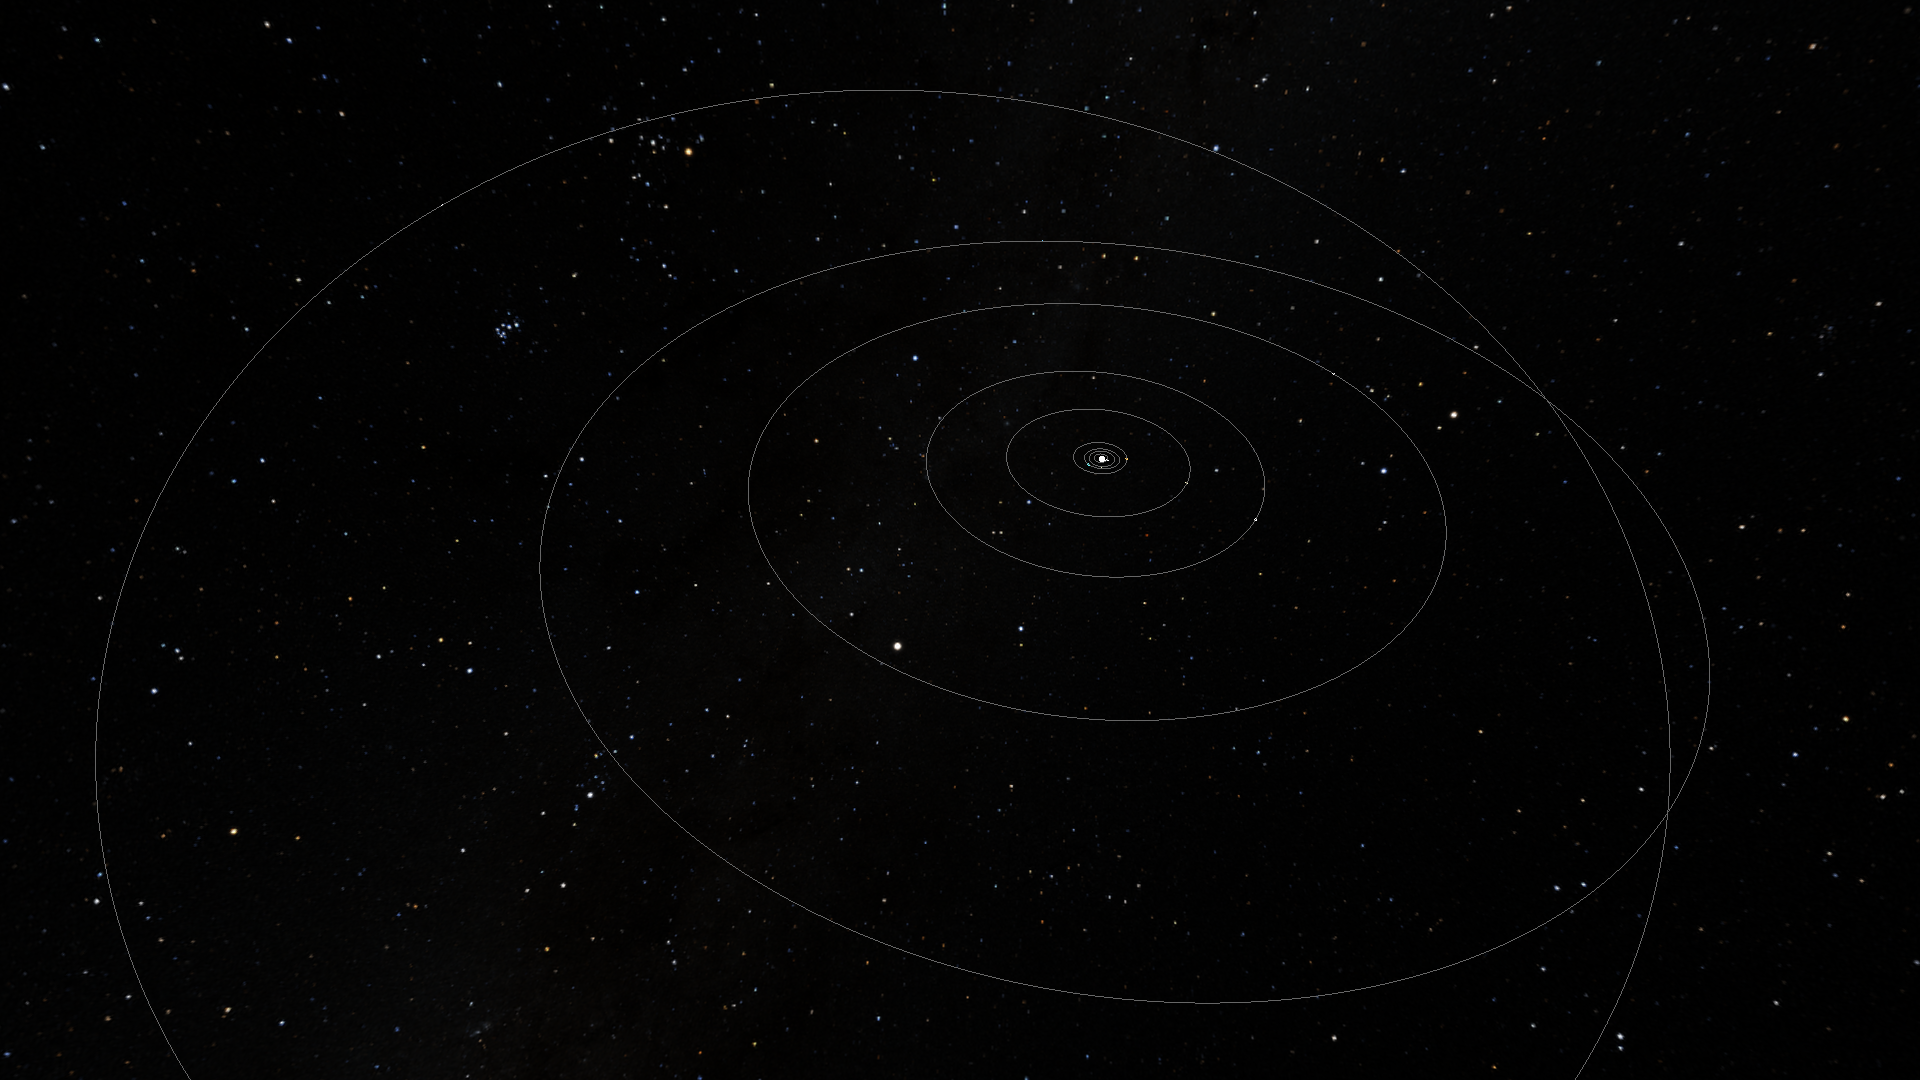
\includegraphics[width=0.95\textwidth]{images/orbits.png}
            \caption{Renderowanie proceduralnych linii orbit idealnie dopasowanych do wyliczonych matematycznie trajektorii planet}
            \label{fig:screen_orbits}
        \end{figure}

        \newpage

        % 5.3.2
        \subsection{System markerów i nawigacja}
         Aby planety były widoczne nawet z dużej odległości, zastosowano system markerów. 
         Są to proste okręgi rysowane wokół pozycji planety. 
         Marker jest skalowany w taki sposób, aby był zawsze zauważalny, ale skalowanie to odbywa się w shaderze lub poprzez macierz modelu markera (\var{model_marker}), która jest niezależna od skali samej planety.

         \bigbreak

         System nawigacji przestrzennej oparto na modelu swobodnej kamery (First Person Camera / Free Look). Znormalizowany wektor kierunku patrzenia wyznaczany jest w oparciu o klasyczne kąty Eulera: odchylenie (\var{yaw}) oraz pochylenie (\var{pitch}), których wartości są dynamicznie modyfikowane na podstawie przesunięć kursora myszy. Aby zapobiec zjawisku odwrócenia kamery i blokady przegubów (tzw. Gimbal Lock w osi pionowej), kąt pochylenia jest algorytmicznie ograniczany do przedziału $[-89^{\circ}, 89^{\circ}]$. 

         Następnie wektor orientacji bocznej (Right) oraz wektor pionu kamery (Up) wyliczane są za pomocą matematycznego iloczynu wektorowego (Cross Product) wektora kierunkowego i stałego wektora „góry” świata (\var{head\_position}). Translacja pozycji kamery odbywa się wzdłuż wyznaczonych w ten sposób wektorów lokalnych za pomocą klawiatury. Implementacja ta, zawarta w funkcjach \func{\_g\_game\_mouse\_handle} oraz \func{\_g\_game\_keyboard\_handle}, pozwala na intuicyjne przemieszczanie się po Układzie Słonecznym.

        % Rysunek 5.2 ""
        \begin{figure}[htpb]
            \centering
            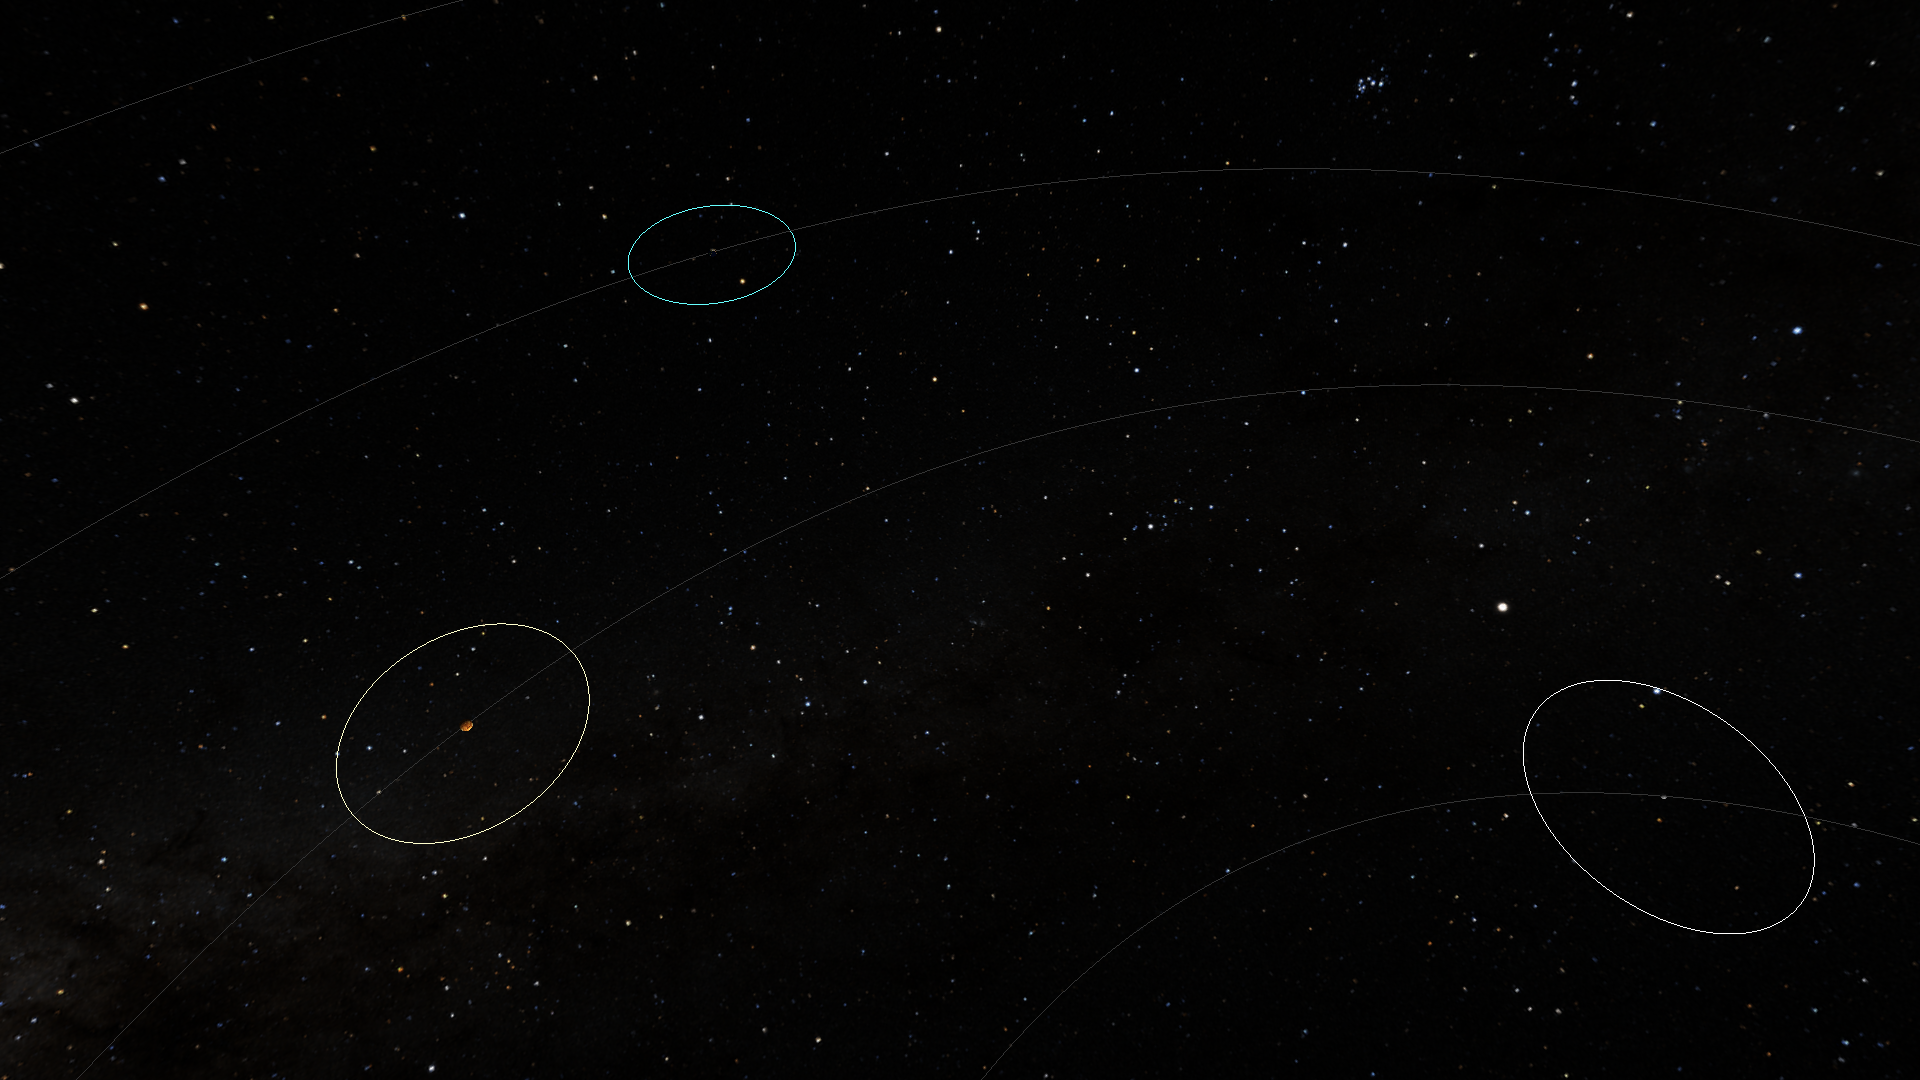
\includegraphics[width=0.95\textwidth]{images/markers.png}
            \caption{System skalowalnych markerów ułatwiający nawigację i lokalizację odległych obiektów w przestrzeni kosmicznej}
            \label{fig:screen_markers}
        \end{figure}
         

% zakończenie
\summary
Celem niniejszej pracy inżynierskiej było zaprojektowanie oraz implementacja interaktywnej wizualizacji Układu Słonecznego „SOLAR”, działającej w czasie rzeczywistym. Założenie to zostało w pełni zrealizowane poprzez stworzenie autorskiego silnika graficznego opartego na standardzie języka C oraz bibliotece graficznej OpenGL 4.1 Core Profile. Projekt udowodnił, że możliwe jest zbudowanie wydajnego, stabilnego i edukacyjnie wartościowego oprogramowania bez uciekania się do wykorzystania gotowych, komercyjnych silników gier, co wymagało jednak głębokiego zrozumienia niskopoziomowych mechanizmów działania potoku renderującego oraz matematyki trójwymiarowej.

W ramach warstwy technologicznej z sukcesem zaimplementowano własną bibliotekę matematyczną do obsługi macierzy i kwaternionów, zrezygnowano ze standardowej, dynamicznej alokacji pamięci na rzecz wysoce zoptymalizowanego mechanizmu alokatora liniowego (Memory Arena) oraz opracowano autorski, binarny format modeli 3D (\file{.orb}). Dzięki stworzeniu dedykowanego narzędzia konwertującego \var{otob}, wykorzystującego algorytm haszujący FNV-1a do deduplikacji wierzchołków, drastycznie zredukowano czas ładowania zasobów oraz zoptymalizowano wykorzystanie pamięci karty graficznej.

W warstwie logicznej symulacji zaimplementowano deterministyczny model mechaniki nieba oparty na parametrach orbitalnych Keplera. Wykorzystanie numerycznej metody Newtona-Raphsona pozwoliło na precyzyjne wyznaczanie pozycji planet w przestrzeni na podstawie równania Keplera, a zintegrowany system czasu umożliwił użytkownikowi płynną manipulację chronologią wydarzeń w skali od pojedynczych sekund do całych lat. Całość została dopełniona interfejsem użytkownika obejmującym proceduralnie generowane linie orbit, zaawansowany system nawigacji przestrzennej (Free Look) oraz dynamicznie skalujące się markery, które rozwiązują problem nawigacji w ogromnej skali kosmicznej.

Przeprowadzone testy działania aplikacji potwierdzają spełnienie wszystkich zdefiniowanych na początku pracy wymagań funkcjonalnych i niefunkcjonalnych. Program utrzymuje płynność renderowania na wysokim poziomie (znacznie powyżej wymaganych 60 klatek na sekundę) nawet przy symulacji całego układu planetarnego, nie wykazuje wycieków pamięci dzięki scentralizowanemu zarządzaniu zasobami, a jego architektura pozostaje wysoce modularna, co ułatwia ewentualną rozbudowę.

\newpage

\vspace{1em}
\noindent \textbf{\Large Możliwe kierunki dalszego rozwoju}
\vspace{0.5em}

Architektura stworzonego silnika stanowi solidny fundament, który w przyszłości może zostać rozbudowany o kolejne, zaawansowane moduły technologiczne i symulacyjne:

\begin{itemize}
    \item \textbf{Implementacja cieni dynamicznych (Shadow Mapping):} Wprowadzenie algorytmów rzutowania cieni z punktowego źródła światła (Słońca) pozwoliłoby na realistyczne symulowanie zjawisk astronomicznych, takich jak zaćmienia planet czy rzucanie cieni przez księżyce na powierzchnie gazowych gigantów.
    
    \item \textbf{Rozszerzenie modelu fizycznego o grawitację n-ciał:} Przejście z deterministycznego, "sztywnego" modelu keplerowskiego na dynamiczną symulację numeryczną (np. z wykorzystaniem integratora Verleta lub metody Rungego-Kutty) umożliwiłoby badanie perturbacji orbitalnych i stabilności nowo dodawanych układów gwiezdnych.
    
    \item \textbf{Proceduralne generowanie atmosfery:} Zastąpienie statycznych tekstur na modelach planet posiadających gęstą atmosferę (Ziemia, Wenus) zaawansowanymi programami cieniującymi (shaderami), realizującymi fizyczne rozpraszanie Rayleigha i Mie. Drastycznie podniosłoby to fotorealizm wizualizacji.
    
    \item \textbf{Implementacja wielowątkowości do ładowania zasobów:} Wykorzystanie systemowych wątków (np. standardu POSIX Threads) do asynchronicznego wczytywania modeli i tekstur w tle. Wyeliminowałoby to ewentualne zacięcia głównej pętli renderującej (stuttering) podczas dynamicznej rozbudowy symulacji o tysiące obiektów, takich jak pasy asteroid.
    
    \item \textbf{Rozbudowa zawartości astronomicznej i interfejsu:} Implementacja algorytmów renderowania czcionek (SDF Fonts) w celu wyświetlania na ekranie precyzyjnych etykiet informacyjnych oraz telemetrycznych układów UI. Ponadto, wygenerowanie tła kosmicznego na podstawie rzeczywistych katalogów gwiazd (np. Hipparcos) zamiast wykorzystania statycznej mapy sześciennej (Skybox).
    
    \item \textbf{System dźwięku przestrzennego:} Integracja lekkiej, niskopoziomowej biblioteki audio (np. OpenAL) w celu dodania udźwiękowienia interfejsu użytkownika oraz symulowania przestrzennych zjawisk dźwiękowych, co znacząco wpłynęłoby na immersję płynącą z użytkowania aplikacji.
\end{itemize}


\printbibliography[type=book,title={Bibliografia - książki}]
\printbibliography[type=article,title={Bibliografia - artykuły}]
\printbibliography[type=online,title={Bibliografia - strony internetowe}]

% spis tabel
\listoftables

% spis rysunków
\listoffigures

% spis listingów
\lstlistoflistings

\end{document}